\begin{frame}
	\myheading{Module 8.6 : Parameter Sharing and tying}
\end{frame}

\begin{frame}
	\vspace{4em}
	\begin{overlayarea}{\textwidth}{\textheight}
		\begin{block}{Other forms of regularization}
			\begin{itemize}
				\item $L2$ regularization
				\item Dataset augmentation
				\item \textcolor<2->{red}{Parameter Sharing and tying}
				\item Adding Noise to the inputs 
				\item Adding Noise to the outputs 
				\item Early stopping
				\item Ensemble methods
				\item Dropout
			\end{itemize}
		\end{block}
	\end{overlayarea}
\end{frame}
		
		
% %% 1- frame is remaining here
\begin{frame}
	\begin{columns}
		\column{0.5\textwidth}
		\vspace{1em}
		\begin{overlayarea}{\textwidth}{\textheight}
			\hspace{2em}
			\vspace{1em}
			\begin{tikzpicture}
	\node[anchor=south west,inner sep=0] at (0,0) 
	{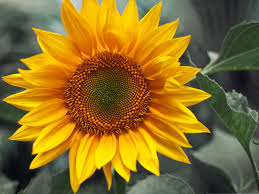
\includegraphics[scale=0.5]{images/flowr.jpg}};
						
	\draw[blue, xstep=.2,ystep=.2] (0,2.4) grid (1,3.4);
	\draw[gray, fill=gray,opacity=0.6] (0,2.4) rectangle (1,3.4);
						
	\draw[blue,xstep=.2,ystep=.2] (3.5,0) grid (4.5,1);
	\draw[gray, fill=gray,opacity=0.6] (3.5,0) rectangle (4.5,1); 
						
	\draw[blue,xstep=.2,ystep=.2] (1.5,1.3) grid (2.5,2.3);
	\draw[gray, fill=gray,opacity=0.6] (1.5,1.3) rectangle (2.5,2.3);
\end{tikzpicture}
								
			\begin{block}<2->{Parameter Sharing}
				\begin{itemize}
					\item<3-> Used in CNNs
					\item<4-> Same filter applied at different positions of the image
					\item<5-> Or same weight matrix acts on different input neurons
				\end{itemize}
			\end{block}
		\end{overlayarea}
						
		\column{0.5\textwidth}
		\vspace{-0.6em}
		\begin{overlayarea}{\textwidth}{\textheight}
			\onslide<6->{
				\tikzstyle{input_neuron}=[circle,draw=red!50,fill=red!10,thick,minimum size=6mm]
\tikzstyle{hidden_neuron}=[circle,draw=blue!50,fill=cyan!10,thick,minimum size=6mm]
\tikzstyle{output_neuron}=[circle,draw=green!50,fill=green!10,thick,minimum size=6mm]
						
\tikzstyle{input}=[circle,draw=black!50,fill=black!20,thick,minimum size=6mm]
						
\begin{center}
	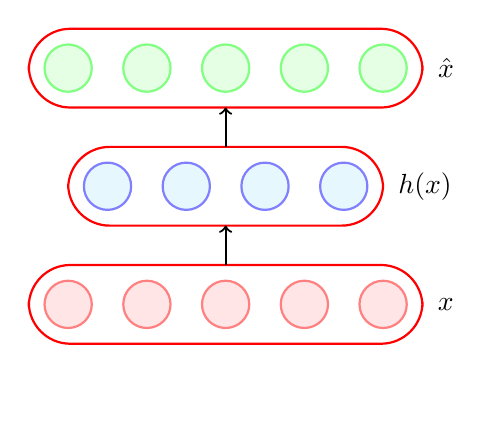
\begin{tikzpicture}
									
		\node (input0) at (6.5,3.5){};
		\node (input1) at (7.5,3.5){};
		\node (input2) at (8.5,3.5){};
		\node (input3) at (9.5,3.5){};
		\node (input4) at (10.5,3.5){};
		\node [input_neuron] (neuron01) at (6.5,4.5) {};
		\node [input_neuron] (neuron02) at (7.5,4.5){};
		\node [input_neuron] (neuron03) at (8.5,4.5) {};
		\node [input_neuron] (neuron04) at (9.5,4.5) {};
		\node [input_neuron] (neuron05) at (10.5,4.5) {};
		\node [hidden_neuron] (neuron51) at (7,6) {} ;
		\node [hidden_neuron] (neuron52) at (8,6)  {};
		\node [hidden_neuron] (neuron53) at (9,6)  {};
		\node [hidden_neuron] (neuron54) at (10,6)  {};
									
		\node [output_neuron] (neuron11) at (6.5,7.5)  {};
		\node [output_neuron] (neuron12) at (7.5,7.5)  {};
		\node [output_neuron] (neuron13) at (8.5,7.5)  {};
		\node [output_neuron] (neuron14) at (9.5,7.5)  {};
		\node [output_neuron] (neuron15) at (10.5,7.5)  {};
									
		\node[text width=0.01cm] at (11.2,4.5) {$x$};
		\node[text width=0.01cm] at (10.7,6) {$h(x)$};
		\node[] at (11.3,7.5) {$\hat{x} $};
		%\node[] at (12.5,7.5) {\footnotesize{$\hat{x}$}};
		\draw[red!100,thick,solid,rounded corners=15pt] (6,4) rectangle (11,5);
		\draw[red!100,thick,solid,rounded corners=15pt] (6.5,5.5) rectangle (10.5,6.5);
		\draw[red!100,thick,solid,rounded corners=15pt] (6,7) rectangle (11,8);
		\draw[thick,->] (8.5,5) -- (8.5,5.5);
		\draw[thick,->] (8.5,6.5) -- (8.5,7);
	\end{tikzpicture}
\end{center}
				\vspace{-1em}
				\begin{block}<7->{Parameter Tying}
					\begin{itemize}
						\item<8-> Typically used in autoencoders
						\item<9-> The encoder and decoder weights are tied.
					\end{itemize}
				\end{block}}
		\end{overlayarea}
	\end{columns}
\end{frame}
